\documentclass[final]{beamer}
  \mode<presentation>
  {
% you can chose your theme here:
\useoutertheme{infolines}
\usetheme{Warsaw}
\useoutertheme{shadow}
\useinnertheme{rounded}
\setbeamertemplate{items}[ball]
\setbeamertemplate{navigation symbols}{}
\setbeamertemplate{blocks}[rounded][shadow=true]
\setbeamertemplate{background canvas}{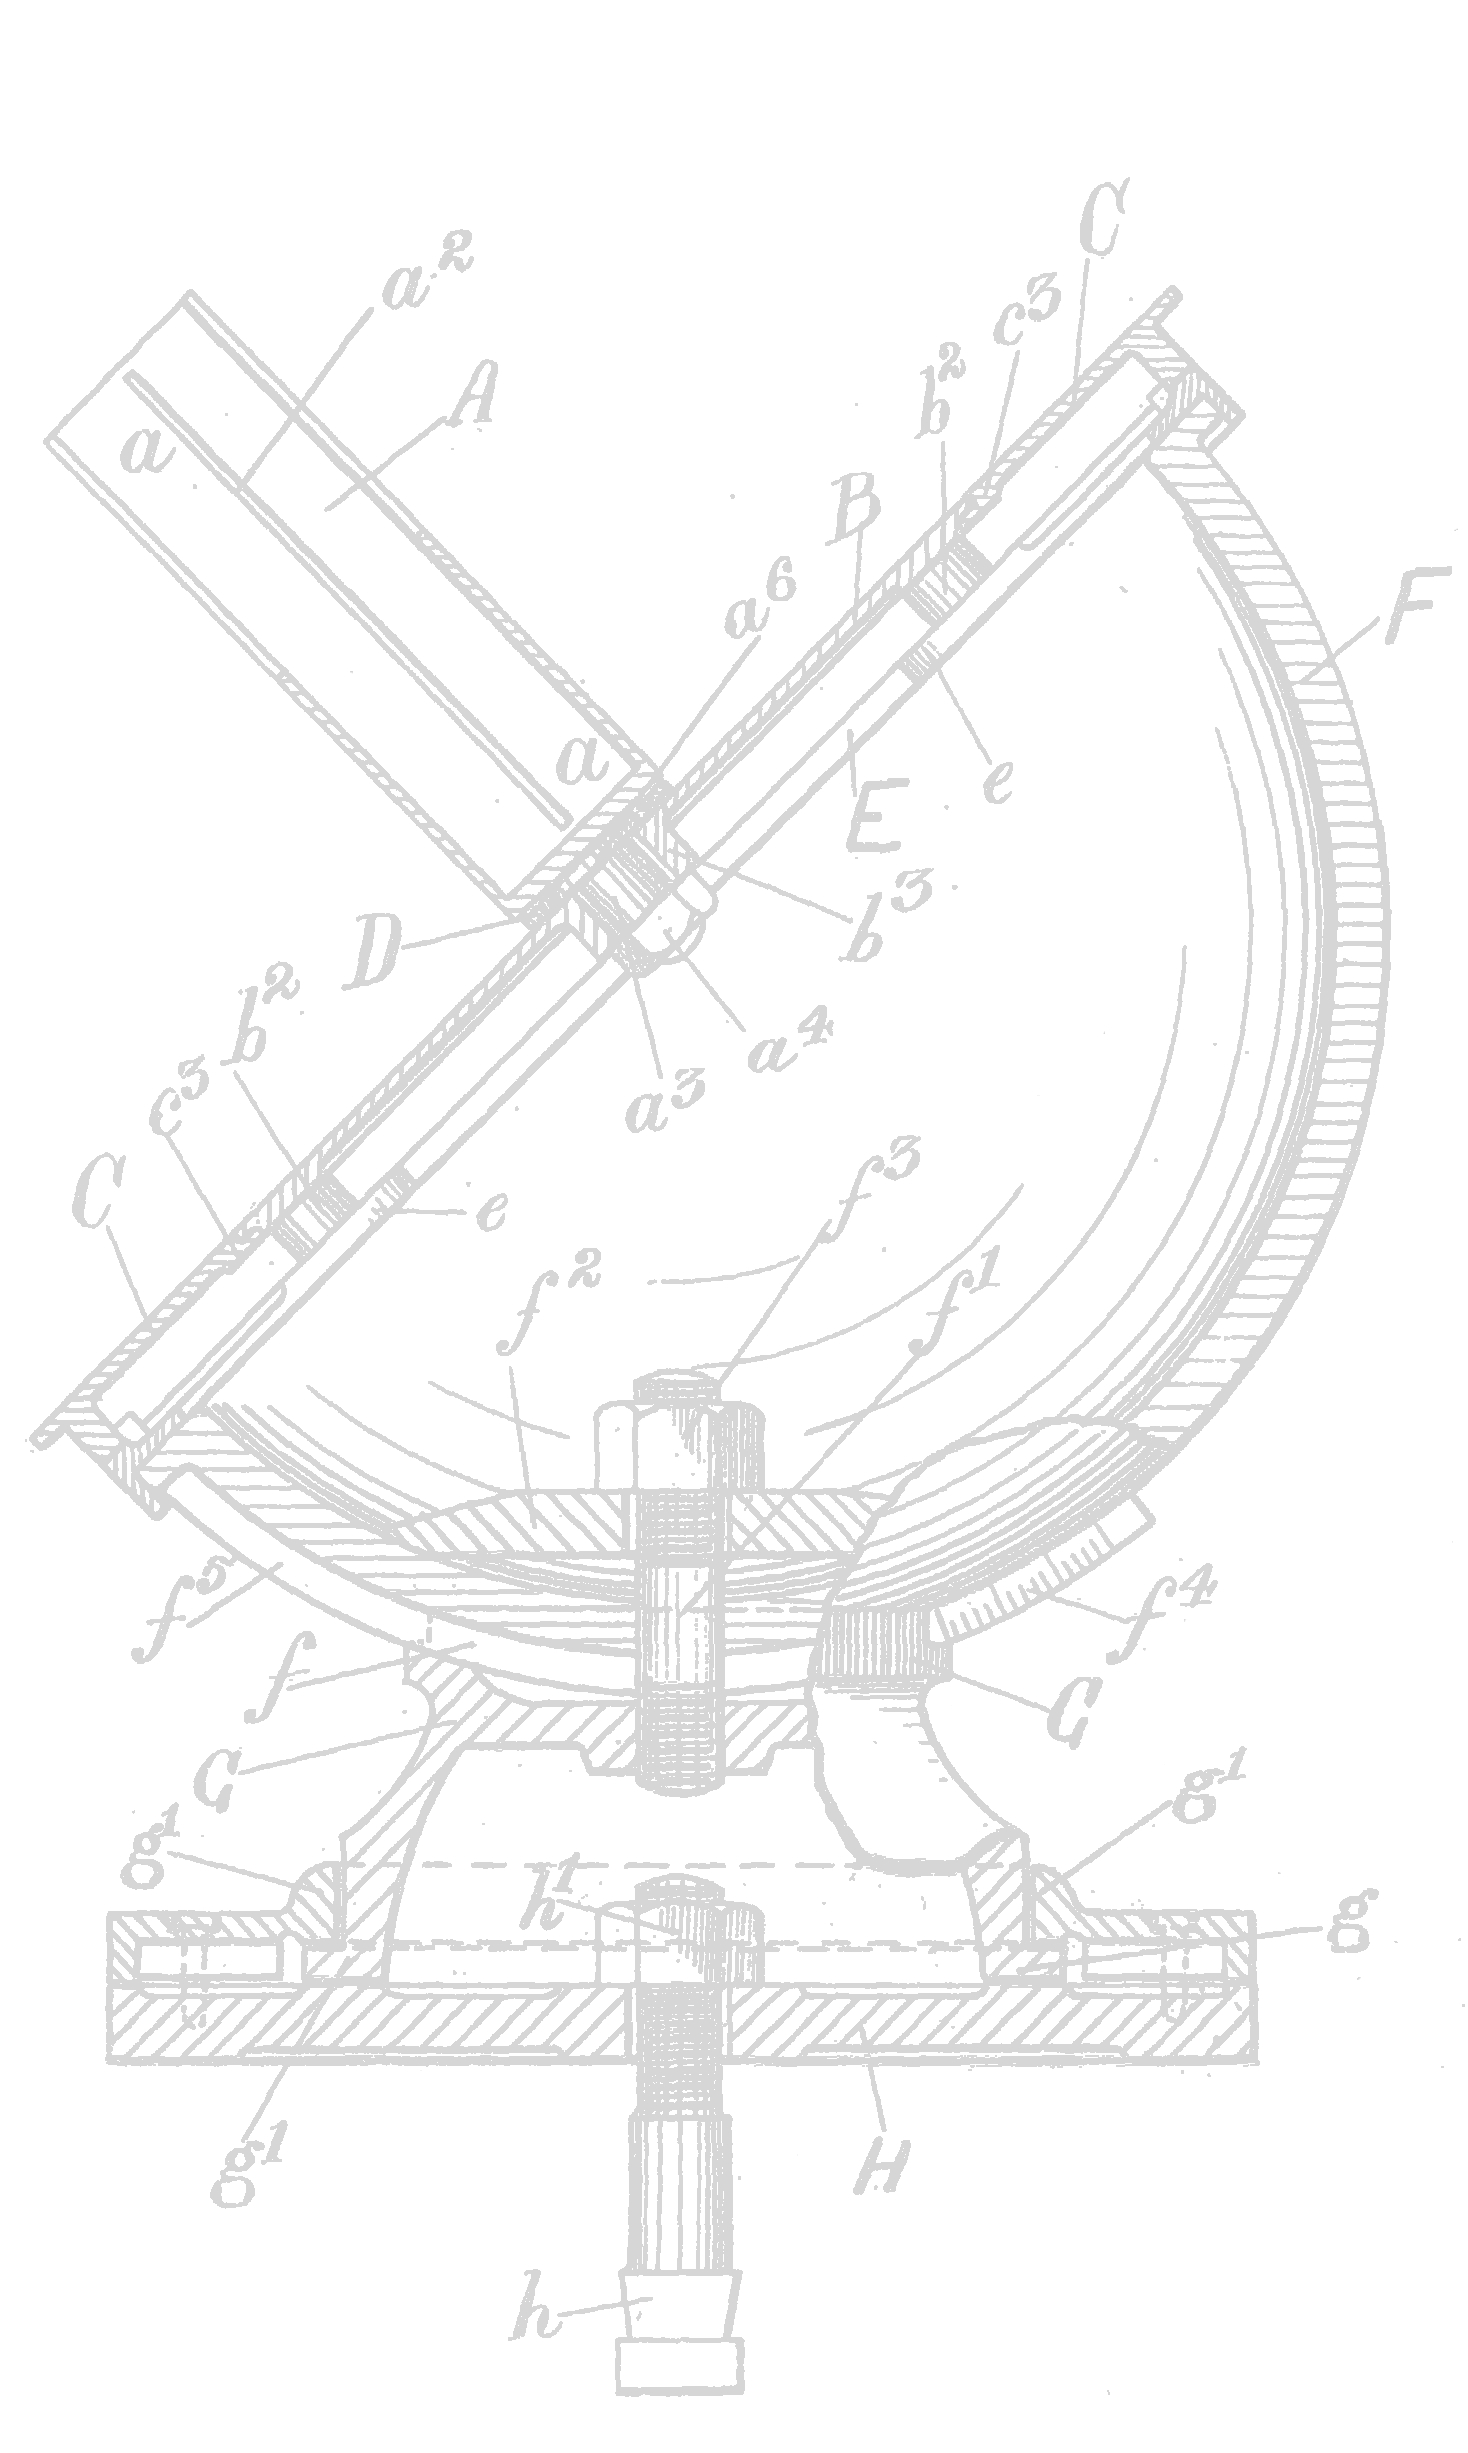
\includegraphics{pilkington2.jpg}
                                      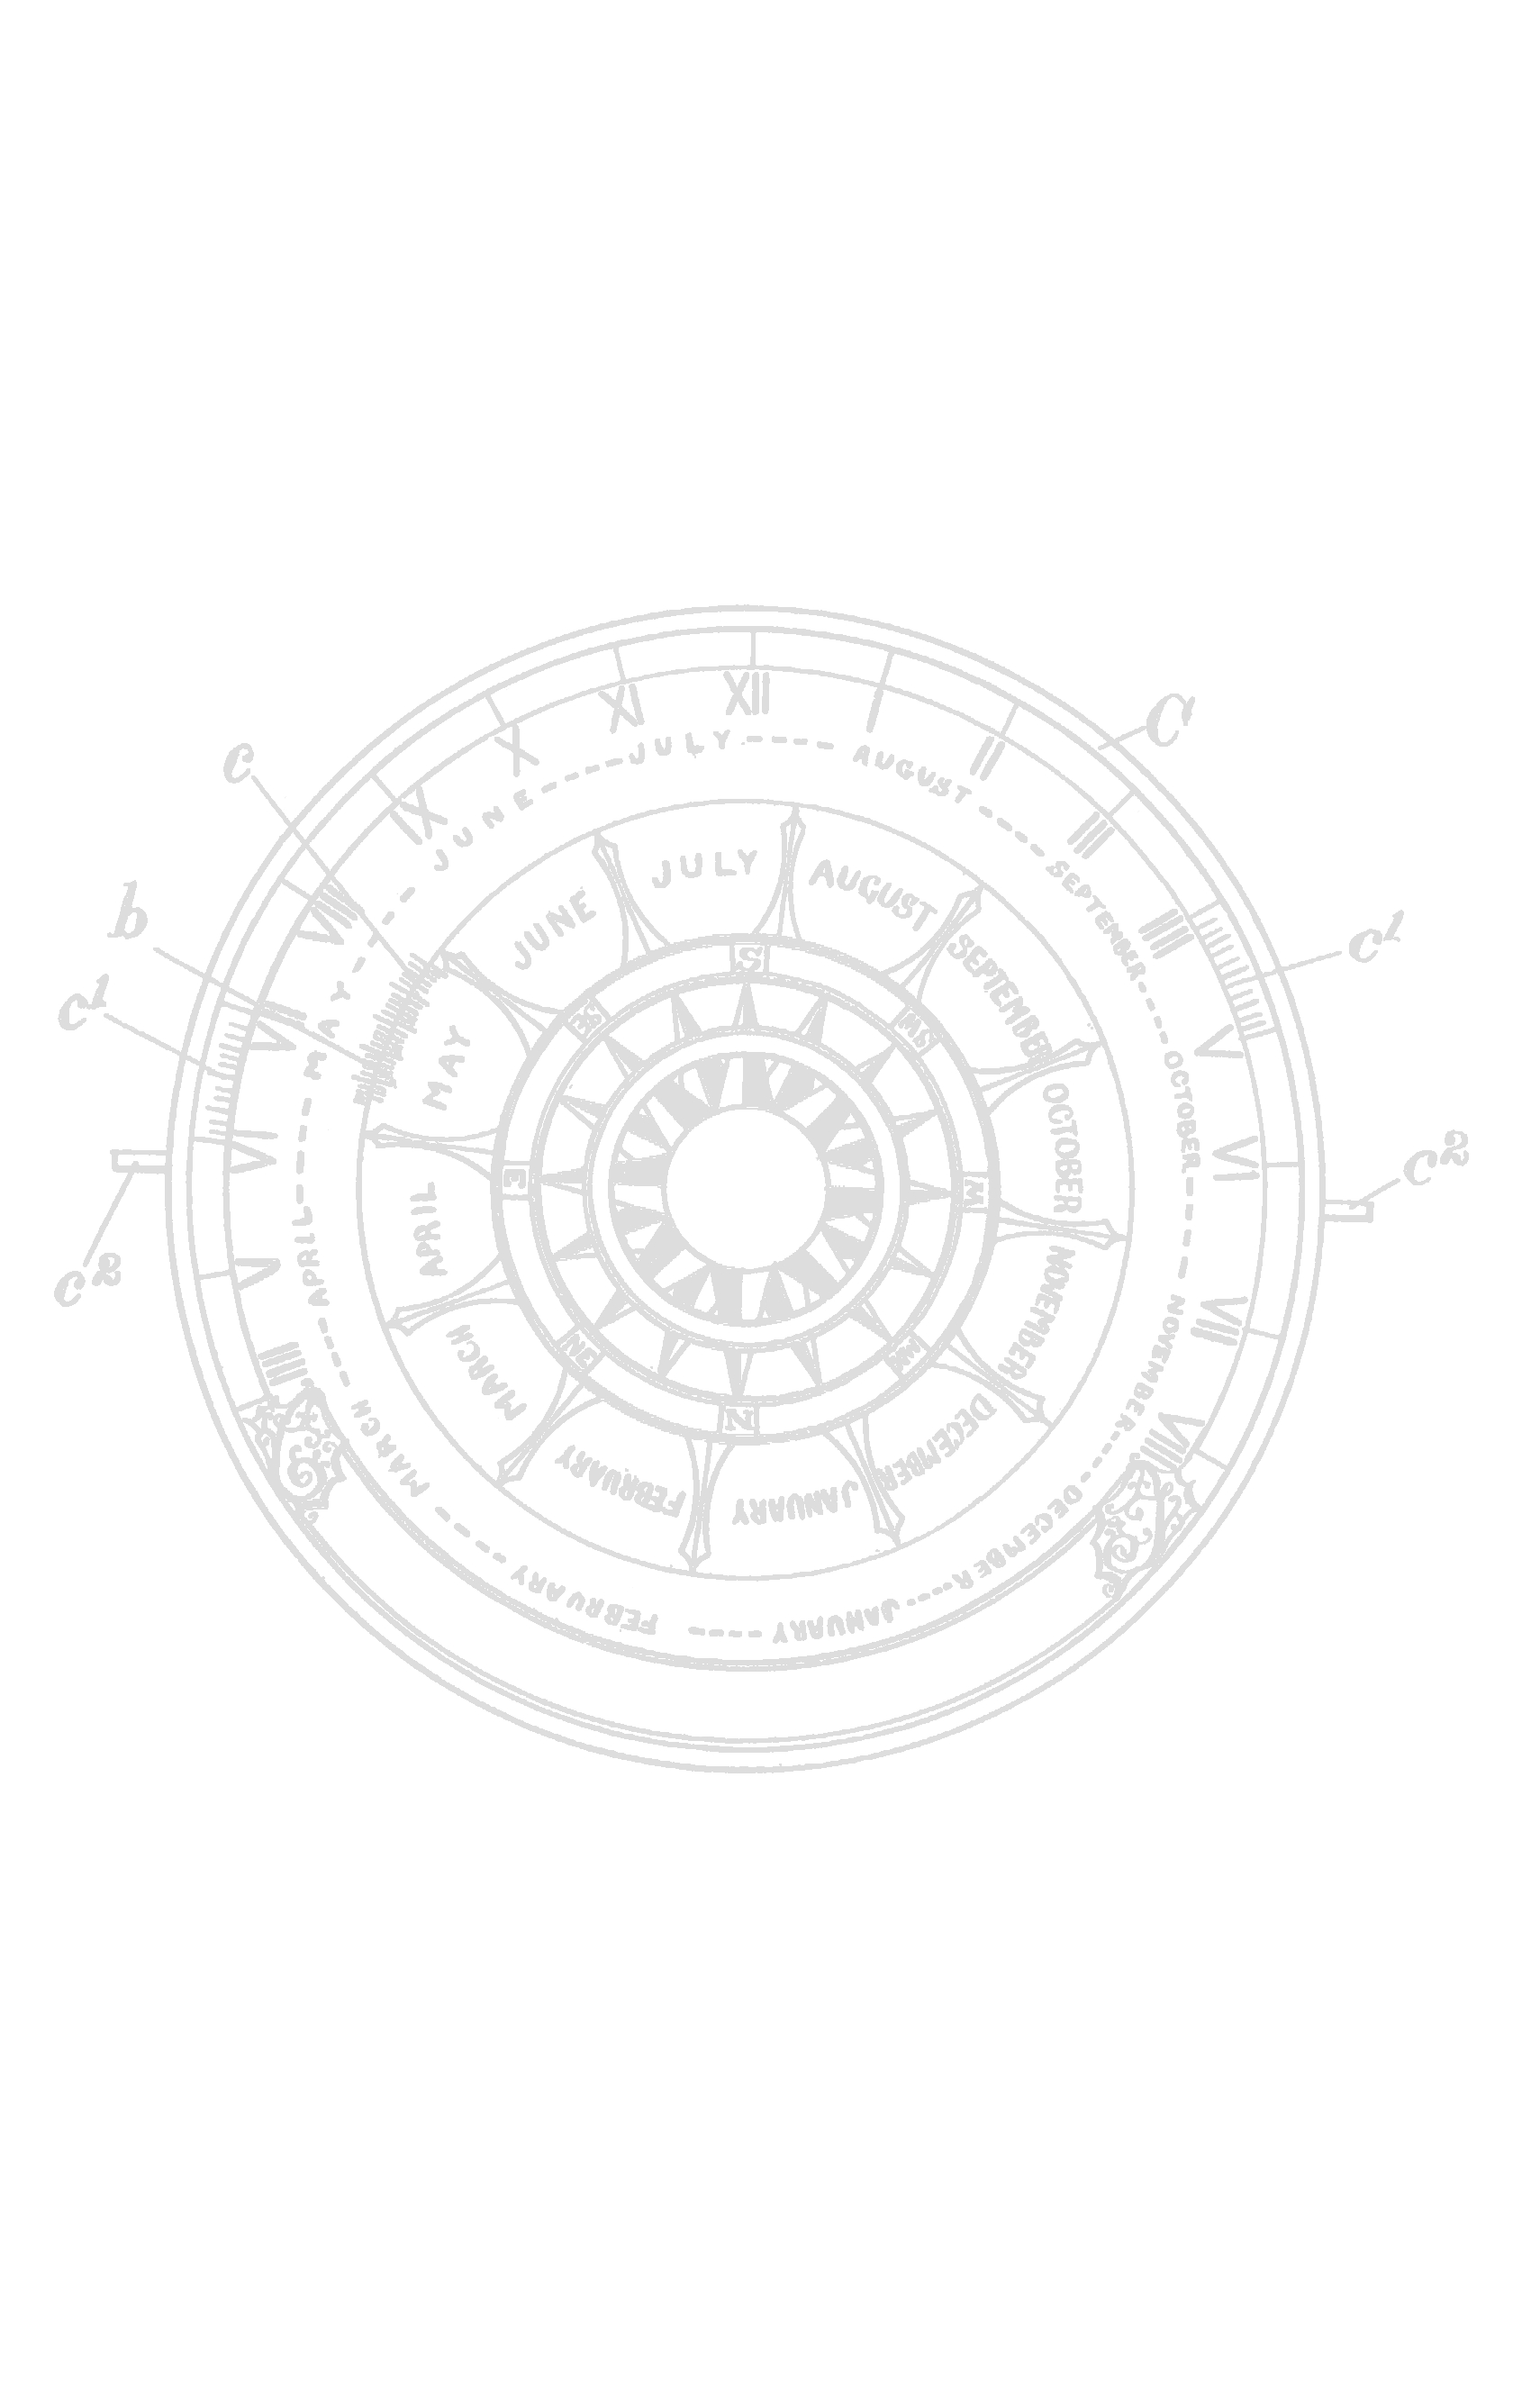
\includegraphics{pilkingtondial.jpg}}
\setbeamerfont{structure}{series=\bfseries} 
\setbeamerfont{frametitle}{size=\VERYHuge}
\setbeamerfont{alerted text}{series=\bfseries}
\setbeamercolor{alerted text}{fg=beamer@blendedblue}

\setbeamertemplate{footline}{
% don't know what leavevmode is but TeX don't like it
%  \leavevmode%
  \hbox{%
  \begin{beamercolorbox}[wd=.42\paperwidth,ht=2.5ex,dp=1.125ex,leftskip=.3cm plus1fill,rightskip=.3cm]{author in head/foot}
    \usebeamerfont{author in head/foot}\insertshortauthor
  \end{beamercolorbox}%
  \begin{beamercolorbox}[wd=.5\paperwidth,ht=2.5ex,dp=1.125ex,leftskip=.3cm,rightskip=.3cm plus1fil]{title in head/foot}%
    \usebeamerfont{title in head/foot}\insertinstitute
  \end{beamercolorbox}%
  \begin{beamercolorbox}[wd=.08\paperwidth,ht=2.5ex,dp=1.125ex,center]{title in head/foot}%
    \insertdate
  \end{beamercolorbox}}%
  \vskip0pt%
}


}

\usepackage{amsmath,amssymb}
\usepackage[english]{babel}
\usepackage[latin1]{inputenc}
\usepackage[orientation=landscape,size=custom,width=111.76,height=86.36,scale=2]{beamerposter}  % e.g. custom size poster
\title{Heliochronometer}
\author{Christopher Maes}
\institute{Mechanical Engineering 203, Stanford University}
\date{December 8th, 2008}


\renewcommand{\tiny}{\fontsize{12}{14}\selectfont}
\renewcommand{\scriptsize}{\fontsize{14.4}{18}\selectfont}   
\renewcommand{\footnotesize}{\fontsize{17.28}{22}\selectfont}
\renewcommand{\small}{\fontsize{20.74}{25}\selectfont}
\renewcommand{\normalsize}{\fontsize{24.88}{30}\selectfont}
\renewcommand{\large}{\fontsize{29.86}{37}\selectfont}
\renewcommand{\Large}{\fontsize{35.83}{45}\selectfont}
\renewcommand{\LARGE}{\fontsize{43}{54}\selectfont}
\renewcommand{\huge}{\fontsize{51.6}{64}\selectfont}
\renewcommand{\Huge}{\fontsize{61.92}{77}\selectfont}
\newcommand{\veryHuge}{\fontsize{74.3}{93}\selectfont}
\newcommand{\VeryHuge}{\fontsize{89.16}{212}\selectfont}
\newcommand{\VERYHuge}{\fontsize{107}{134}\selectfont}

%\newcommand{\titlesize}{\VeryHuge}
%\newcommand{\authorsize}{\LARGE}
%\newcommand{\instsize}{\Large}
       
\setlength\smallskipamount{6pt plus 2pt minus 2pt}
\setlength\medskipamount{12pt plus 4pt minus 4pt}
\setlength\bigskipamount{24pt plus 8pt minus 8pt}
\setlength\abovecaptionskip{25pt}
\setlength\belowcaptionskip{0pt}
\setlength\abovedisplayskip{25pt plus 6pt minus 15 pt}
\setlength\abovedisplayshortskip{0pt plus 6pt}
\setlength\belowdisplayshortskip{13pt plus 7pt minus 6pt}

\pdfpageattr{/Group << /S /Transparency /I true /CS /DeviceRGB>>}
\begin{document}
\begin{frame}
\frametitle{The Heliochronometer} 
\begin{columns}[t]
\begin{column}[t]{0.24 \textwidth}
\alert{What is a heliochronometer?}

\begin{itemize}
\item A {\bf heliochronometer} is a sundial that tells {\bf
standard mean time} by computing a correction from {\bf local real
time} via a mechanical mechanism.

\item 
Standard mean time is the time we use in everyday life, where all
hours have the same length regardless of the season. Regular
sundials tell local real time which is determined directly by
the motion of the sun (when the sun is at its highest it is noon in
local real time).

\item  The heliochronometer uses information such as 
the observer's latitude and longitude, the position of 
true north, as well celestial mechanics and an astronomical
formula called {\bf the Equation of Time} to compute 
standard mean time.
\end{itemize}
    
\alert{History of the heliochronometer}
\begin{itemize}
\item  The heliochronometer was invented by James Gibbs around 1906

\begin{center}
\scalebox{.35}{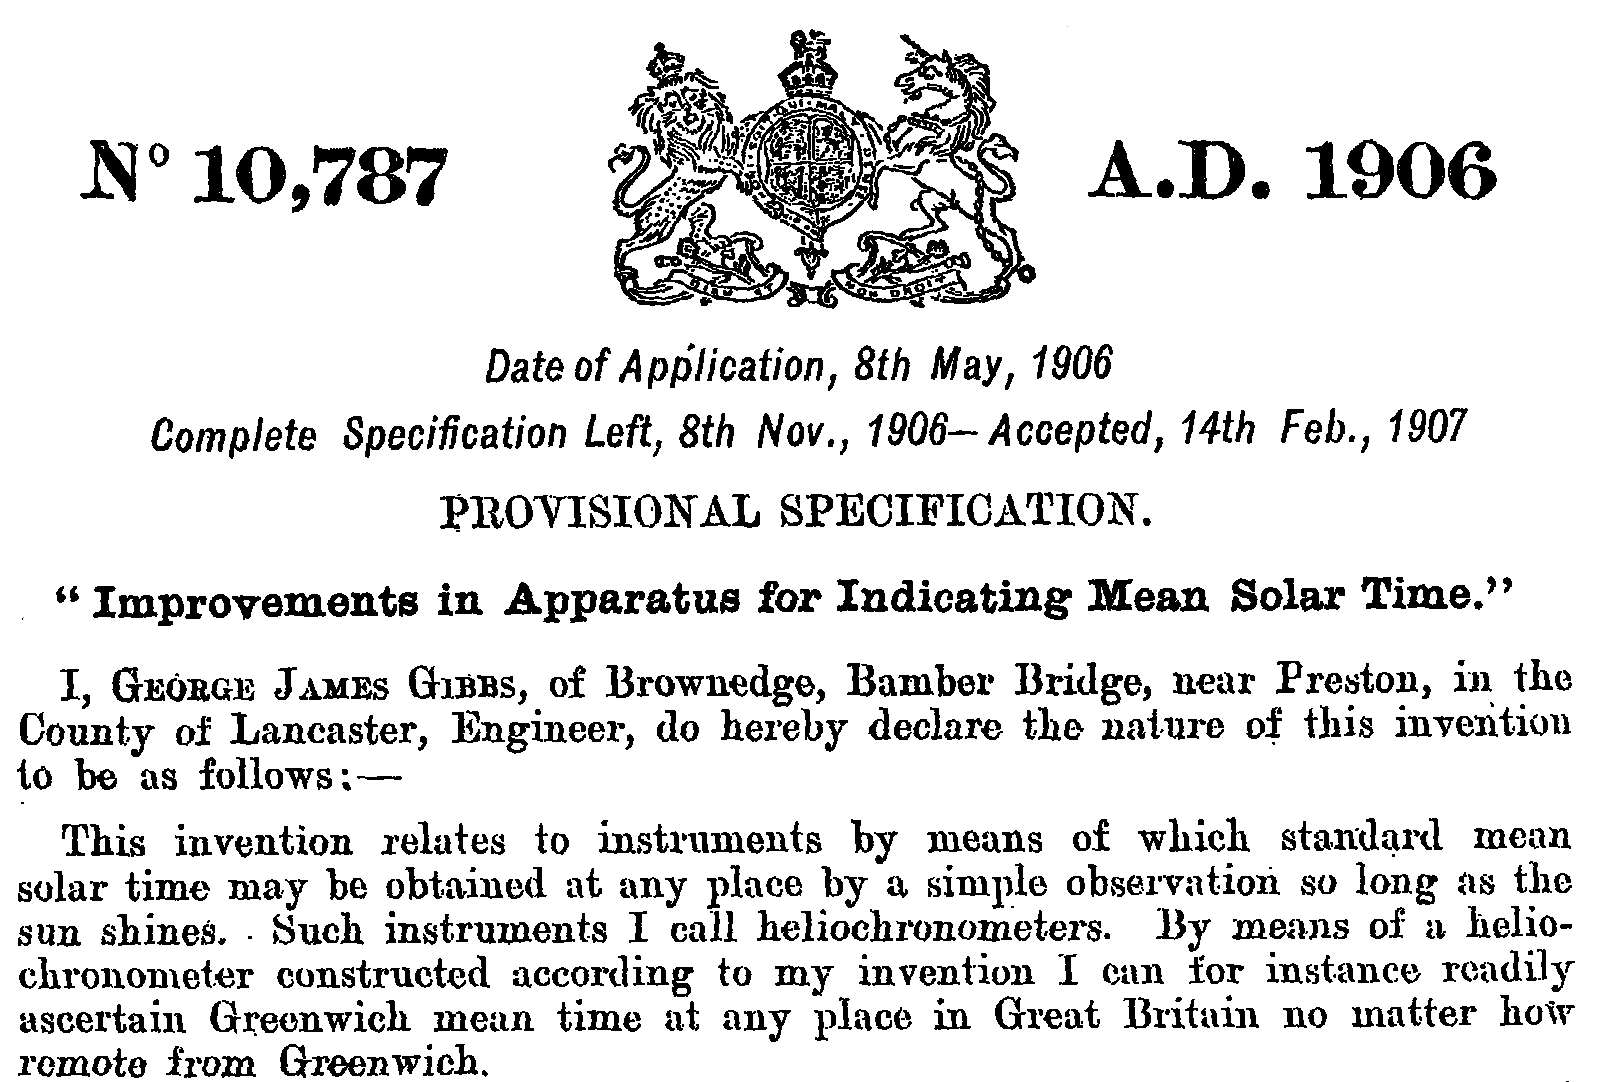
\includegraphics{gibbspatentheader.png}}
\end{center}

\item The heliochronometer solved the need to set mechanical
  wristwatches all over England to Greenwich mean time 

\begin{center}
\scalebox{.5}{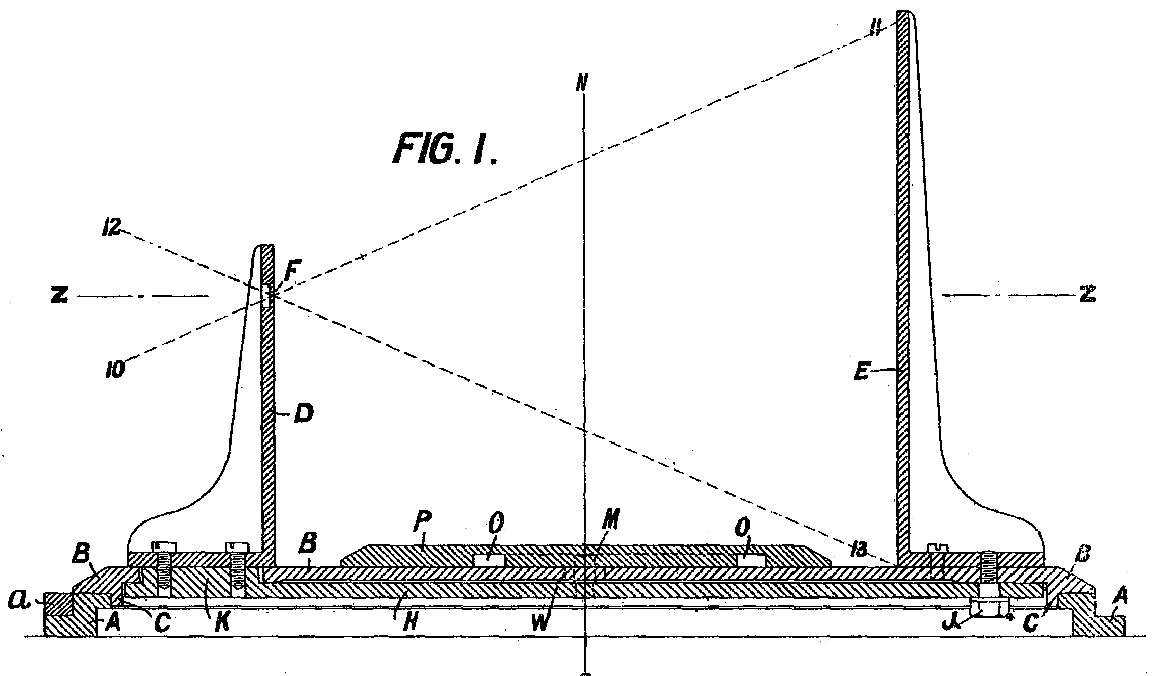
\includegraphics{gibbshelio.png}}
\end{center}

\item Gibbs partnered with William Pilkington to produce the 
{\bf Pilkington \& Gibbs Heliochronometer}


\item Less than a thousand \mbox{P \& G} Heliochronometers were
  made, of which about fifty exist today

\item Original \mbox{P \& G} Heliochronometers are still accurate today, over a hundred years later
\end{itemize}

\vspace*{.5in}

\alert{Why build a heliochronometer today?}
\vspace*{.5in}\\

\emph{ The heliochronometer is an elegant mechanical device. It is
  more than a simple machine. It is a device to mark the hours, an
  optical instrument, and a mechanical computer. Embedded within the
  heliochronometer is the motion of our plant around the sun. Its body
  is aligned with the cardinal directions and its angles tuned to this
  location. When you align the sight with the sun's rays you begin to
  understand the place you occupy in our solar system.  }
\vspace*{1in}

\alert{The anatomy of the modern heliochronometer}

\begin{center}
\scalebox{.2}{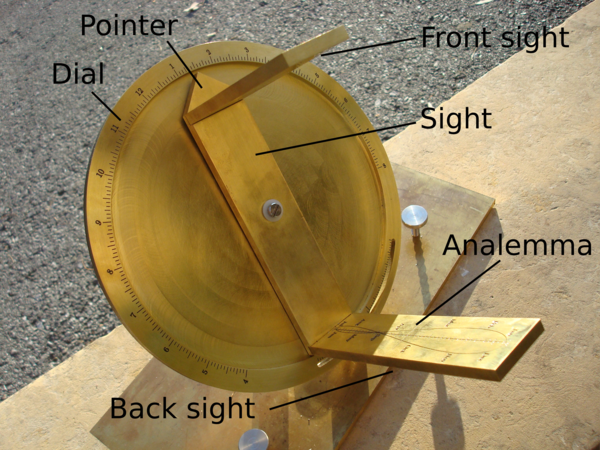
\includegraphics{labeledhelio.png}}
\end{center}


\end{column}

\begin{column}[t]{0.24 \textwidth}
\alert{How does the heliochronometer tell time?}

To compute standard mean time the heliochronometer makes use of
several pieces of information: the observer's latitude, the
hour angle of the sun, the observer's longitude, the direction of true
north, the month of the year, and the declination of the sun.


\begin{itemize}
\item To tell the time the heliochronometer needs to be able 
to precisely located the sun within a reference coordinate system

\item The heliochronometer uses the Equatorial coordinate system.
The sun is located via two angular measurements $\tau$ and $\delta$
\begin{itemize}
\item The hour angle $\tau$ is the angle between the meridian and 
the star measured on the equator
\item The declination $\delta$ is the angular distance from the equator
\end{itemize}

\begin{center}
\scalebox{2.5}{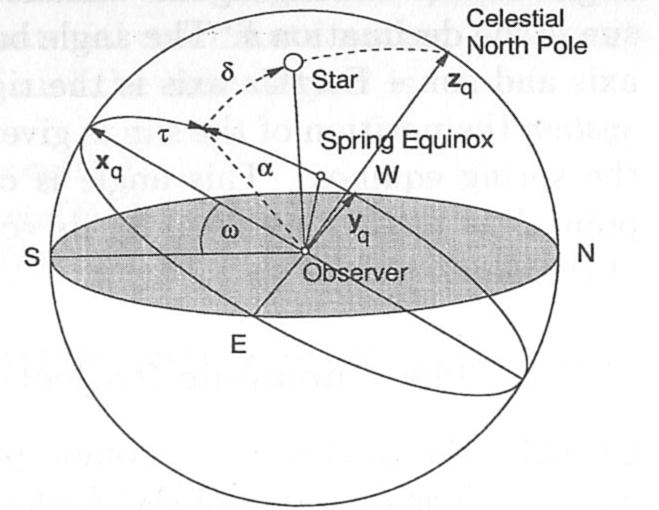
\includegraphics{equatorial.png}}
\end{center}


\item  The angle stands that support the dial have been manufactured so that
the dial lies in a plane parallel to the equator.  The angle $\omega$ is 
the colatitude and $\phi$ is Palo Alto's latitude $37.43 ^\circ$.
\begin{center}
\scalebox{.6}{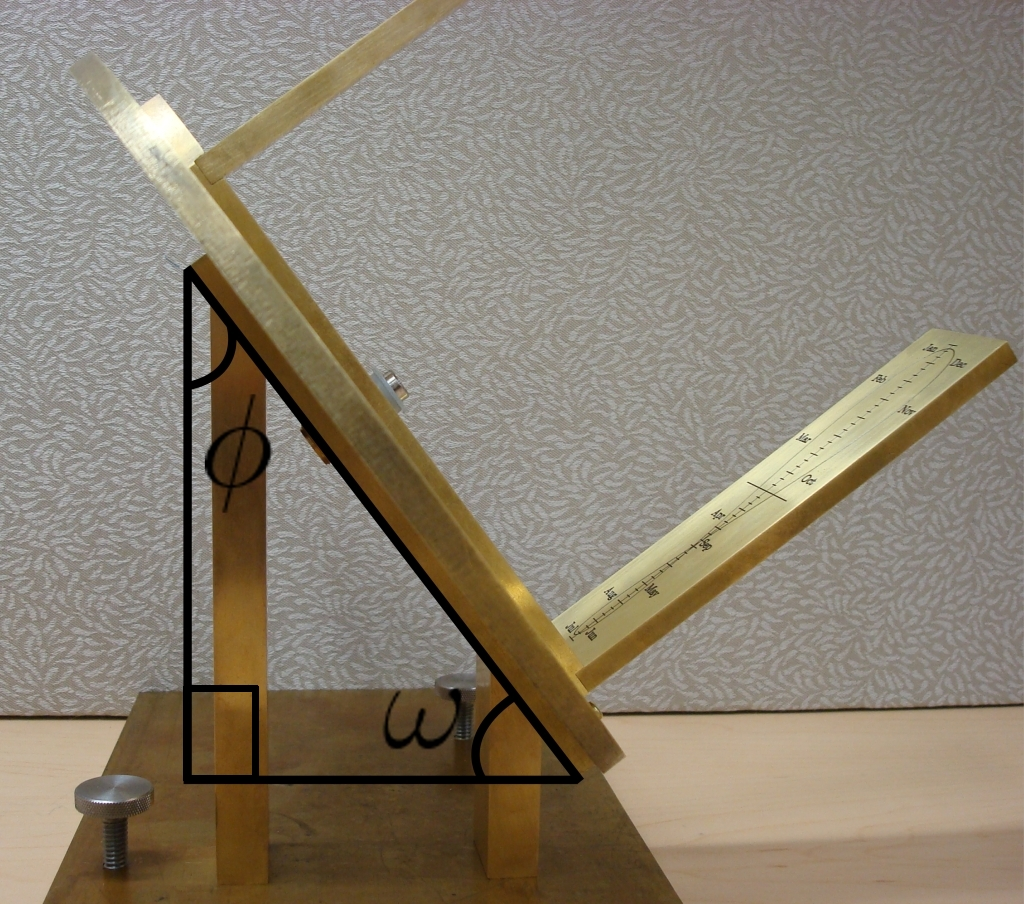
\includegraphics{latangle.jpg}}
\end{center}

\item The base of the dial is rotate so that the angle stands are aligned
with the meridian. The smaller block faces toward north and the larger block 
faces south.

\begin{center}
\scalebox{.2}{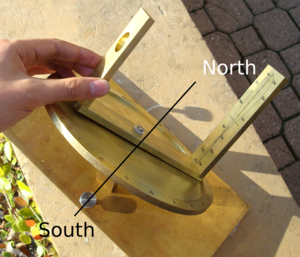
\includegraphics{northsouthalignment.png}}
\end{center}

\item When the sight is rotated so that the sun's light travels
through the pinhole in the front sight and hits the center of the
back sight the pointer measures the angle $\tau$
\begin{center}
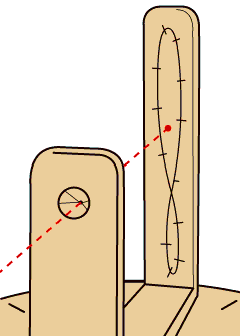
\includegraphics{dialcenter.png}
\end{center}
\item The angle $\tau$ is proportional to the local real time
\begin{center}
\scalebox{.2}{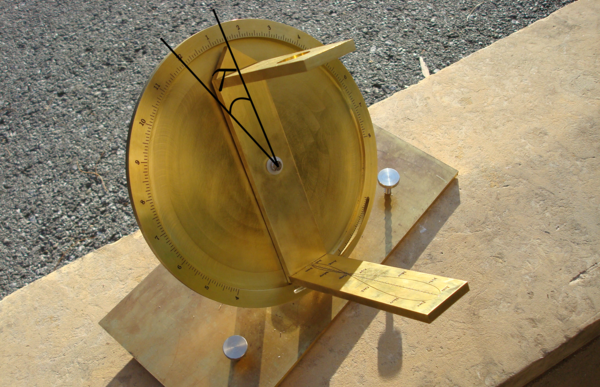
\includegraphics{tauangle.png}}
\end{center}
\end{itemize}




\end{column}
\begin{column}[t]{0.24 \textwidth}
\alert{Converting local real time to standard mean time}
\begin{itemize}
\item Longitude and Time Zones\\
\begin{itemize}
\item The earth is divided into time zones each approximately $15 ^\circ$ degrees of 
longitude wide
\item Under standard mean time the time within a time zone is that of a reference meridian. 
For the Pacific Time Zone the reference meridian is at $120^\circ$ W Longitude. Palo 
Alto is at $122^\circ$ W Longitude.
\item From the perspective of an observer west of the reference meridian the 
sun appears to be slow by four minutes per degree of longitude
\begin{center}
\scalebox{1.25}{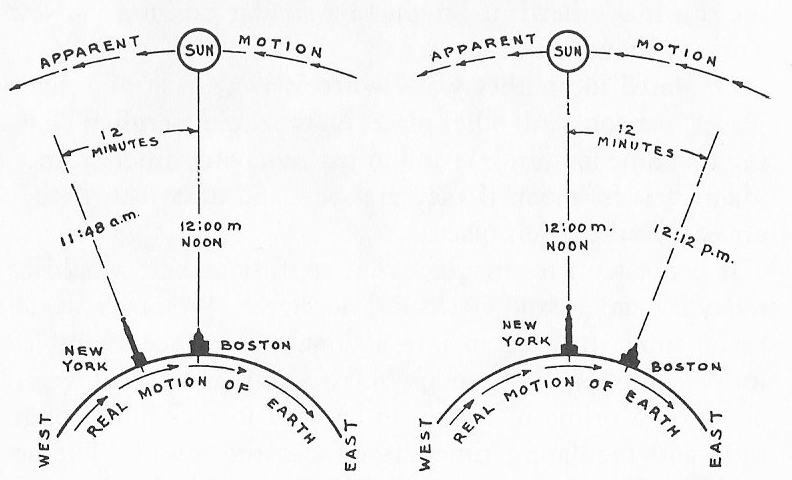
\includegraphics{longitude.png}}
\end{center}
\end{itemize}
\item To adjust for this effect the dial is rotated by the longitudinal offset from
the reference meridian and locked into place with the circumference screw
\begin{center}
\scalebox{.25}{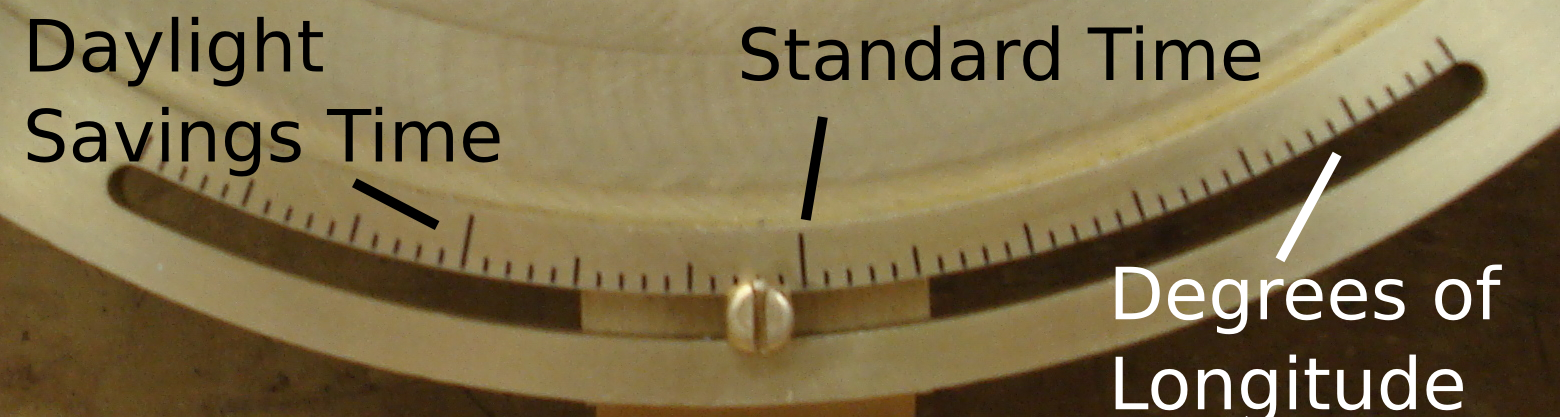
\includegraphics{circumferencescrew.png}}
\end{center}
\item Daylight Savings Time
\begin{itemize}
\item From March to November clocks are adjusted forward one hour for
  Daylight Savings Time. To adjust for DST the dial is rotated
  $15^\circ$. The longitudinal offset is then based off the daylight
  savings time mark rather than the standard time mark.
\end{itemize}
\item The Equation of Time
\begin{itemize}
\item The Equation of Time is an astronomical formula for the difference
between local real time and standard mean time over the course of the 
year
\item The difference is due to two effects: the eccentricity of the 
Earth's orbit and the obliquity of the Earth's rotational axis
\begin{center}
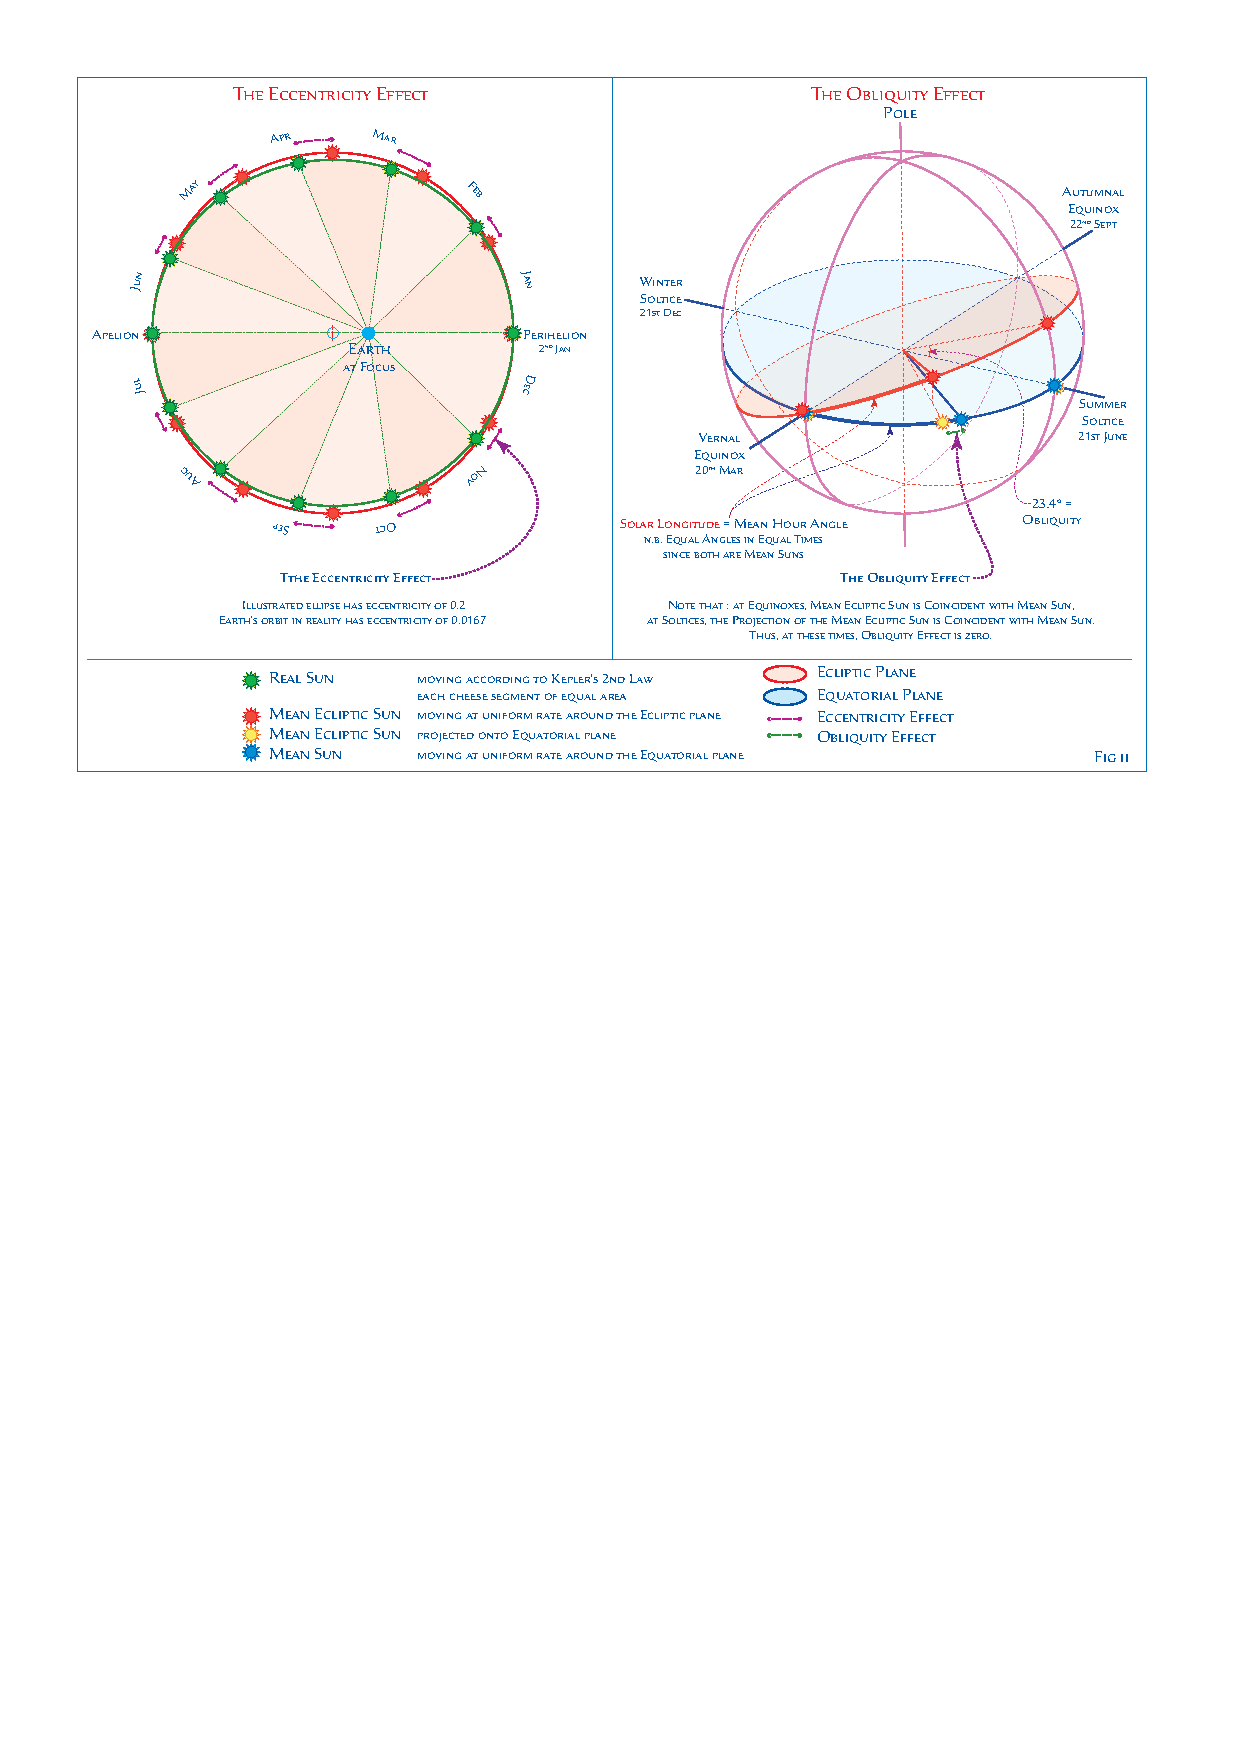
\includegraphics{meansun.pdf}
%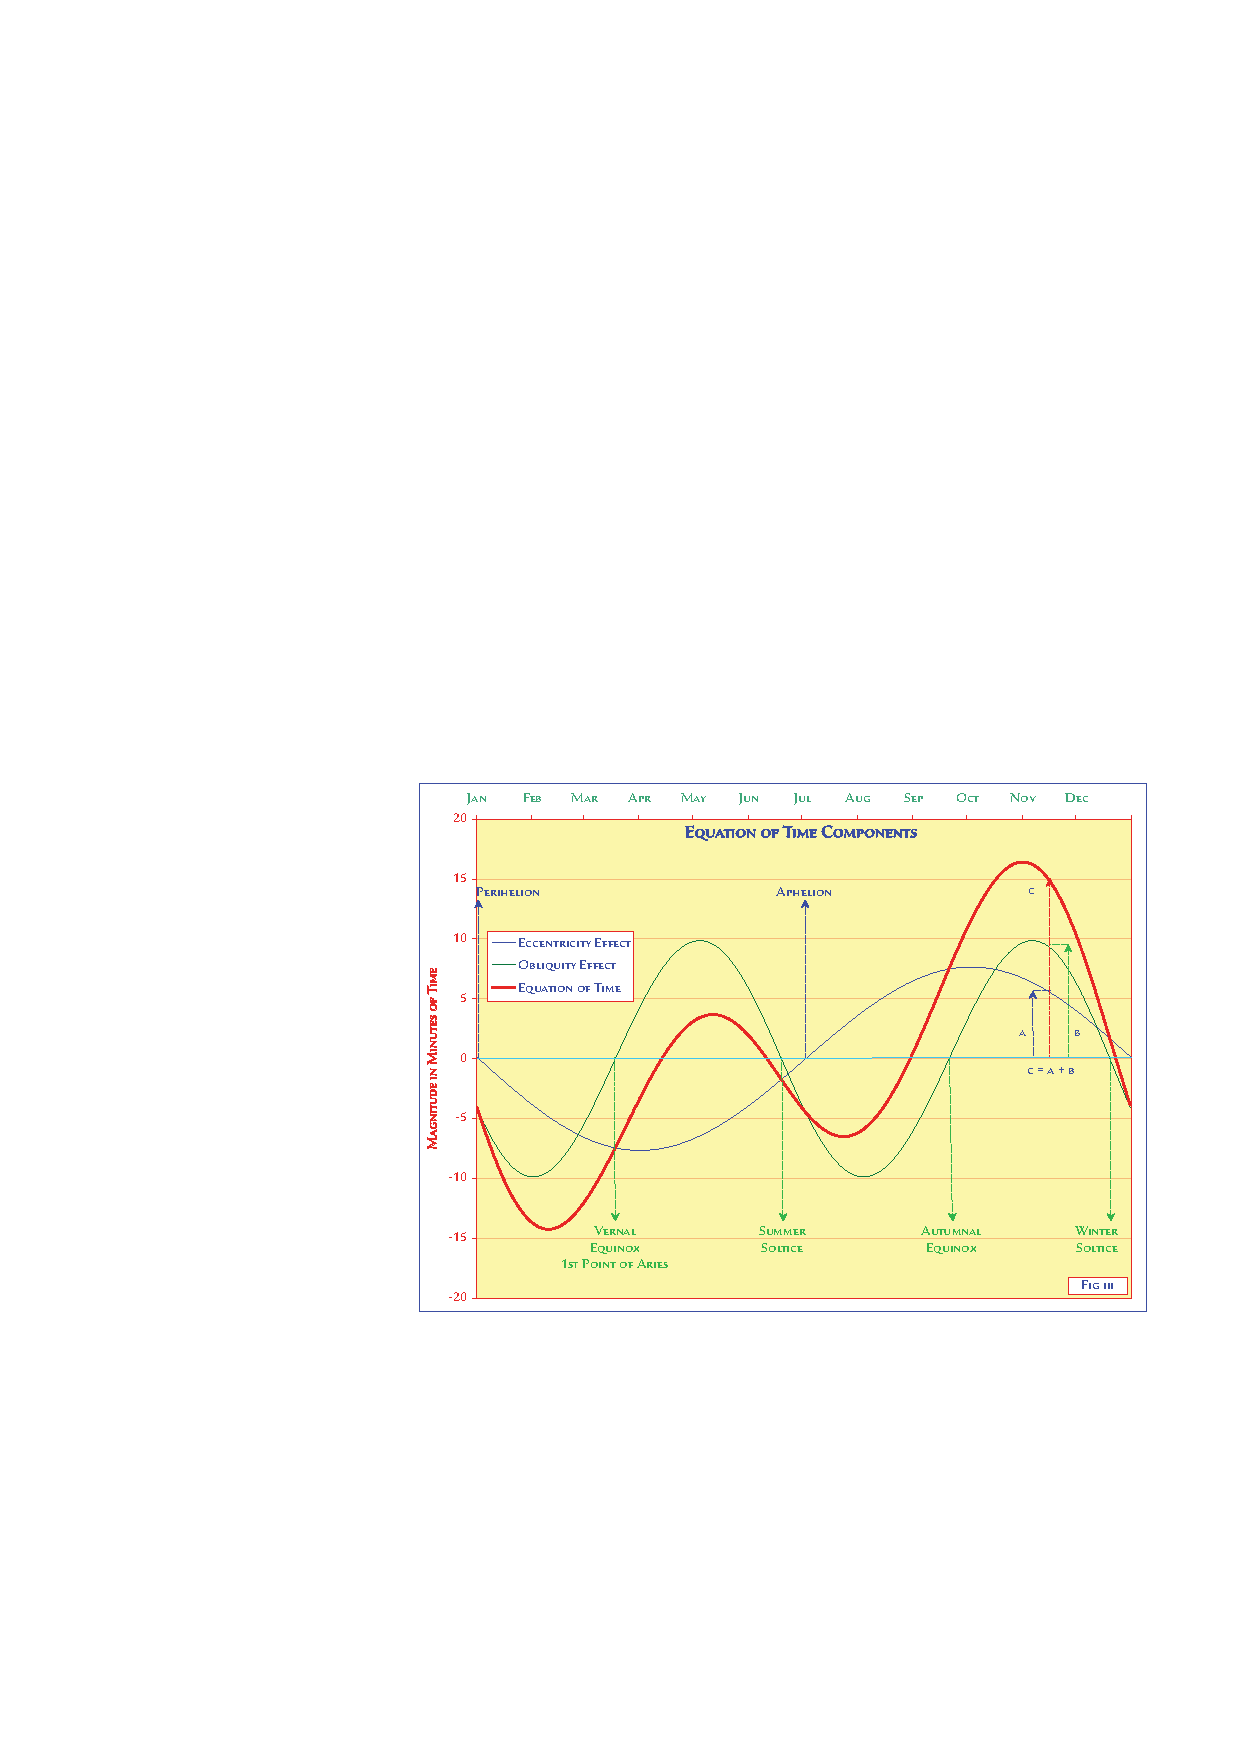
\includegraphics{equationoftimecomponents.pdf}
\end{center}
\end{itemize}
\item The Analemma
\begin{itemize}
\item The engraving on the back sight is a curve 
called the {\bf analemma} that adjusts for the equation of time
\item The vertical axis is the sun's negated declination $-\delta$
\item The horizontal axis is the correction from local real
to standard time due to the equation of time
\begin{center}
\scalebox{.25}{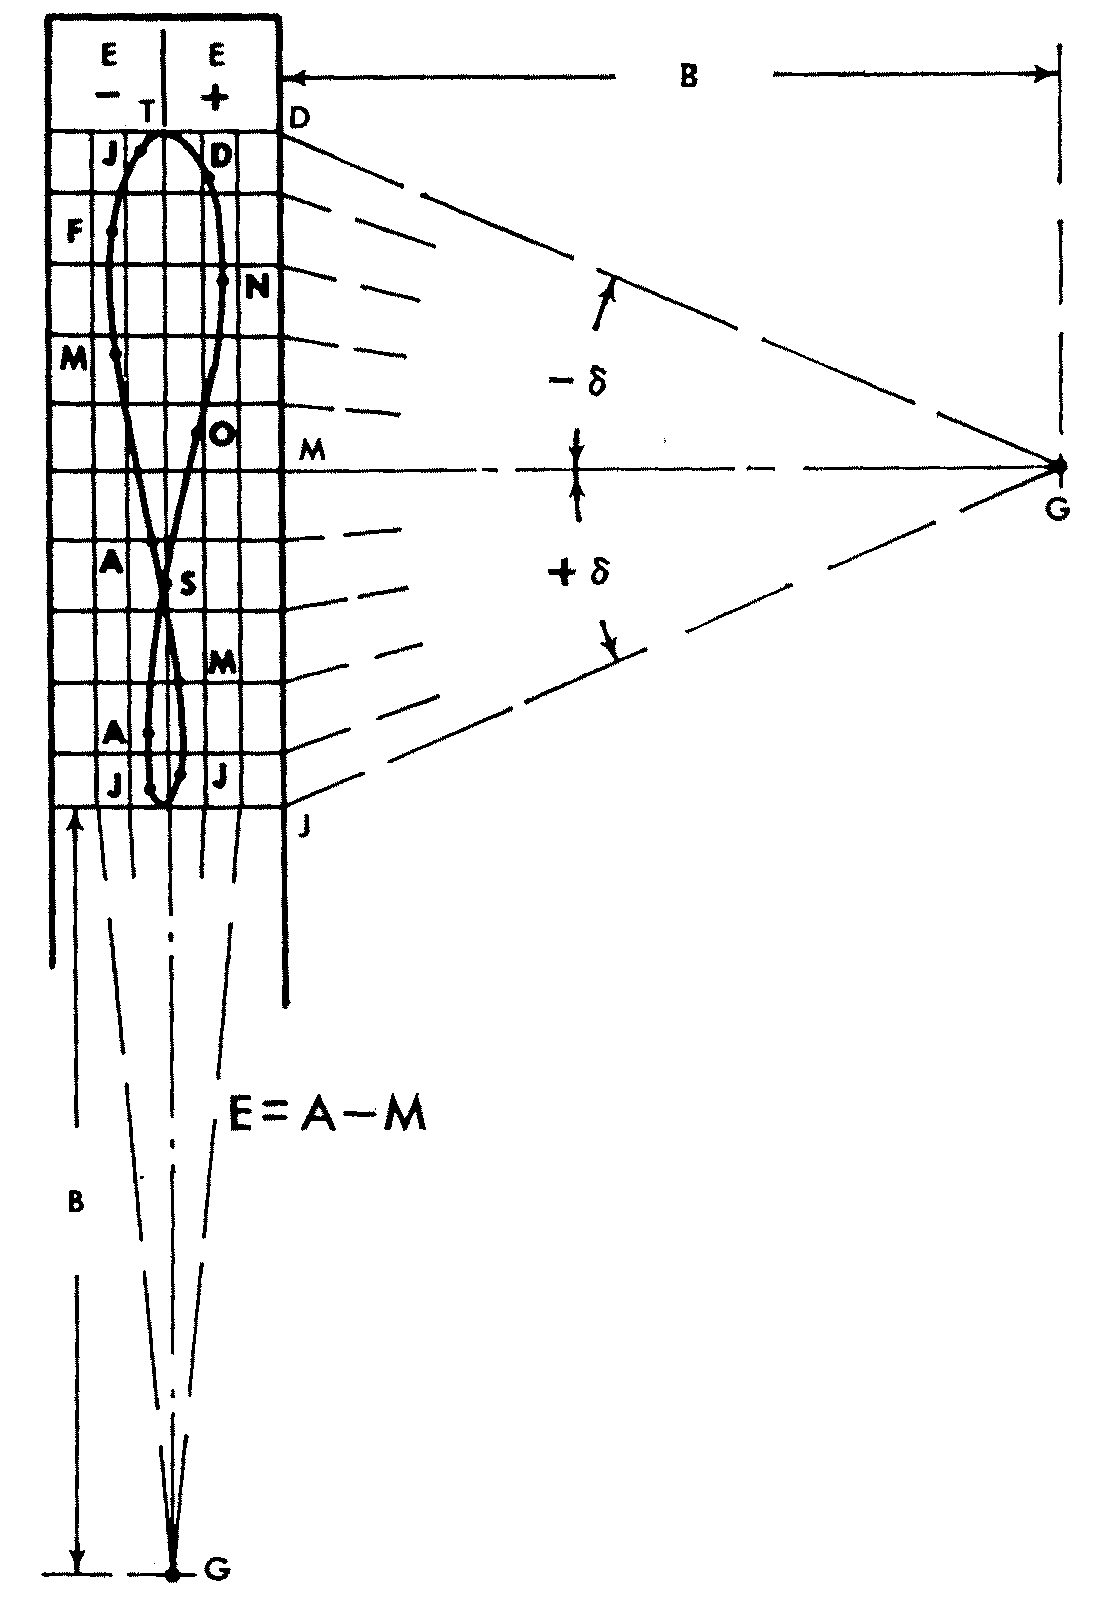
\includegraphics{analemmamayallblack.png}}
\end{center}
\item To compute standard mean time rotate the sight so
that the beam of light is centered on the portion of the 
analemma corresponding to the current month of the year
\begin{center}
\scalebox{.38}{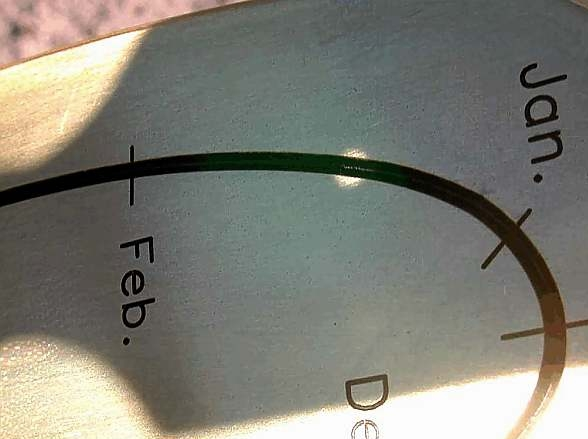
\includegraphics{solardot.jpg}}
\end{center}
\item The analemma can also be seen by taking a picture
of the sun each day at noon over the course of a year
\begin{center}
\scalebox{.38}{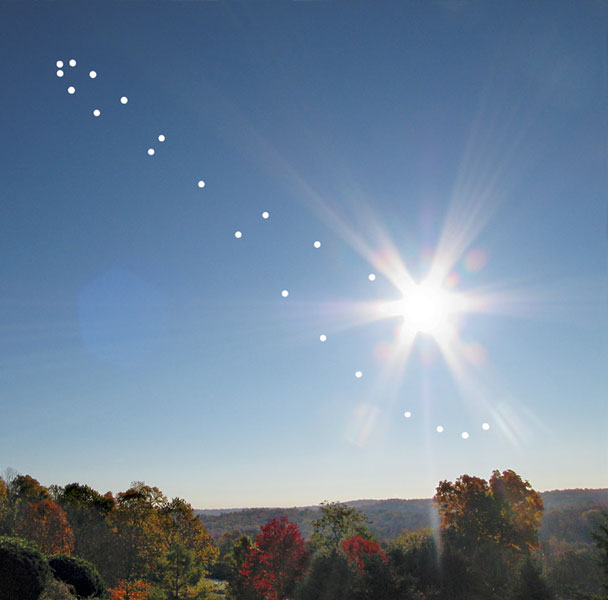
\includegraphics{analemmasun.jpg}}
\end{center}
\end{itemize}
\end{itemize}
\end{column}    

\begin{column}[t]{0.24 \textwidth}
\alert{Design}

\begin{itemize}
\item The design of the heliochronometer is based entirely off the
1906 and 1911 patents, a 1923 sundial construction treatise, and
pictures of similar bespoke heliochronometers made by two modern
craftsmen
\item A significant amount of the design work involved reverse
engineering these previous heliochronometers
\item The sights and pointer were designed using numerical
  optimization. A nonlinear program with ten variables and ten
  constraints was used to find a design that maximized the distance
  between the two sights, subject to constraints imposed by the 
  analemma, the width of the pointer and the inner radius of the dial.
\item A complete CAD model of the heliochronometer was constructed 
including each of the eight hidden fasteners.
\begin{center}
\scalebox{.4}{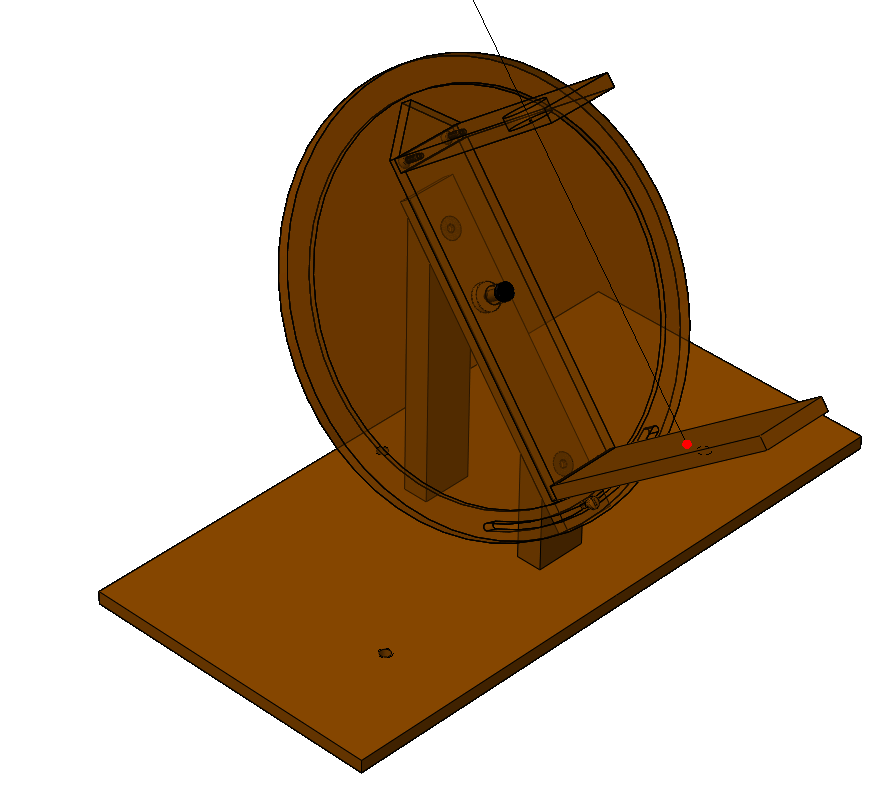
\includegraphics{assemblyscreenshot3.png}}
\scalebox{.4}{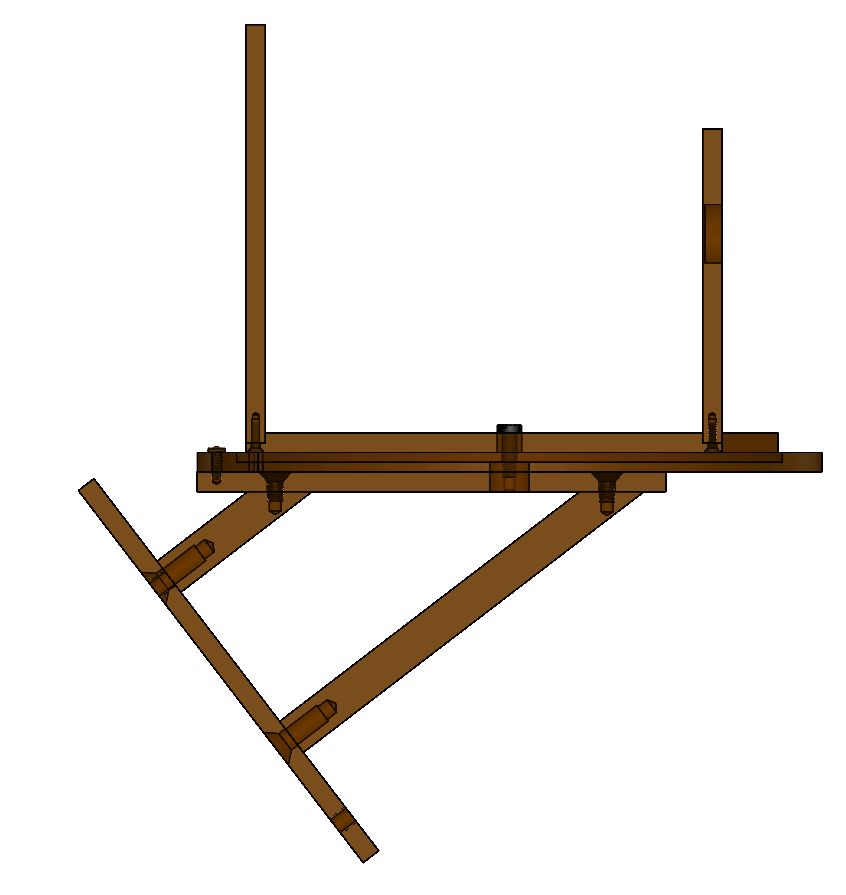
\includegraphics[width=\textwidth]{assemblyscreenshot4.png}}
\end{center}
\end{itemize}


\alert{Manufacturing}

\begin{itemize}
\item Nine brass parts were manufactured on the milling machine,
  rotary table and lathe: the dial plate, the dial support plate, the
  tall latitude angle stand, the short latitude angle stand, the front
  sight, the back sight, the pointer, the concentric rotation half
  threaded rod, and the base plate
\item Two additional acrylic parts were constructed for fixturing:
  a $37.43^\circ$ angle block for machining the latitude angle stands,
  and a alignment plate for engraving the dial. These were made on the
  LaserCAMM.
\item The most difficult parts to manufacture were the dial plate and the 
hidden concentric rotation half-threaded rod 
\begin{itemize}
\item The dial plate was manufactured on the rotary table. It took
several session to machine and had to fixtured and centered 
before each session
\begin{center}
\scalebox{.15}{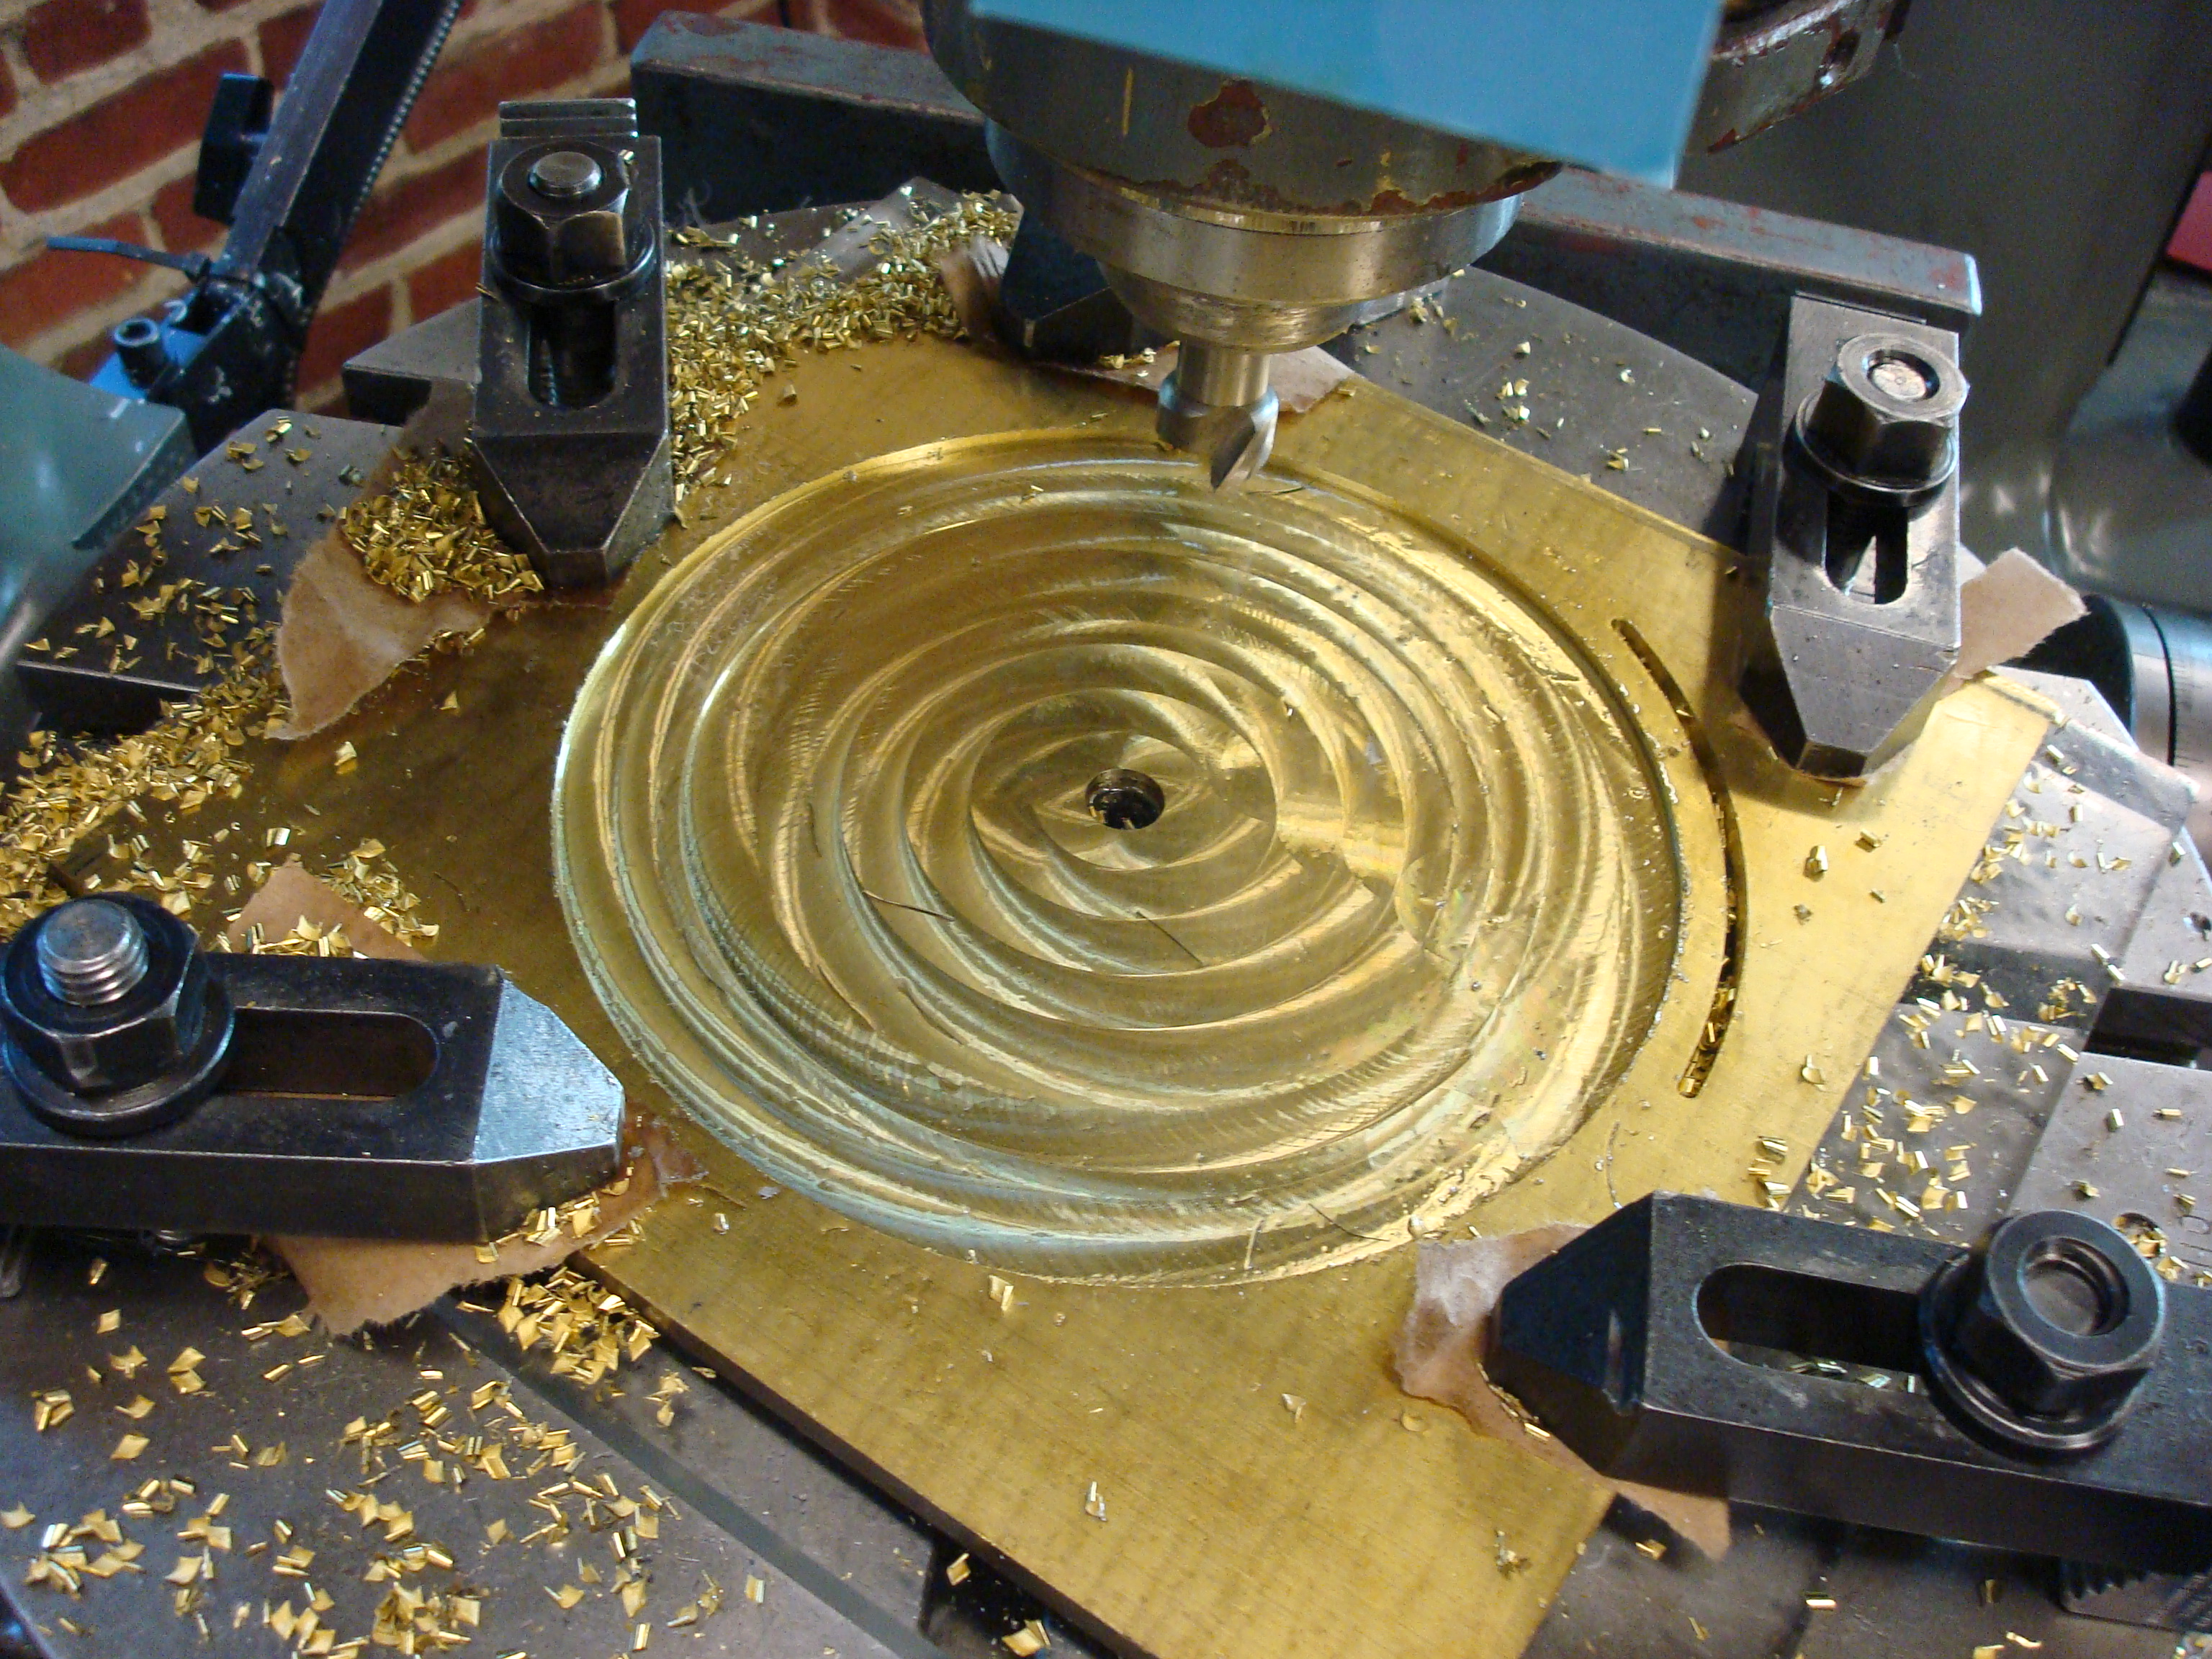
\includegraphics{dialrotarytable.jpg}}\\
\end{center}
\item The half-threaded rod that enables concentric rotation of 
the dial and sight was difficult to machine due to its small size
and its internal and external threads
\begin{center}
\scalebox{.15}{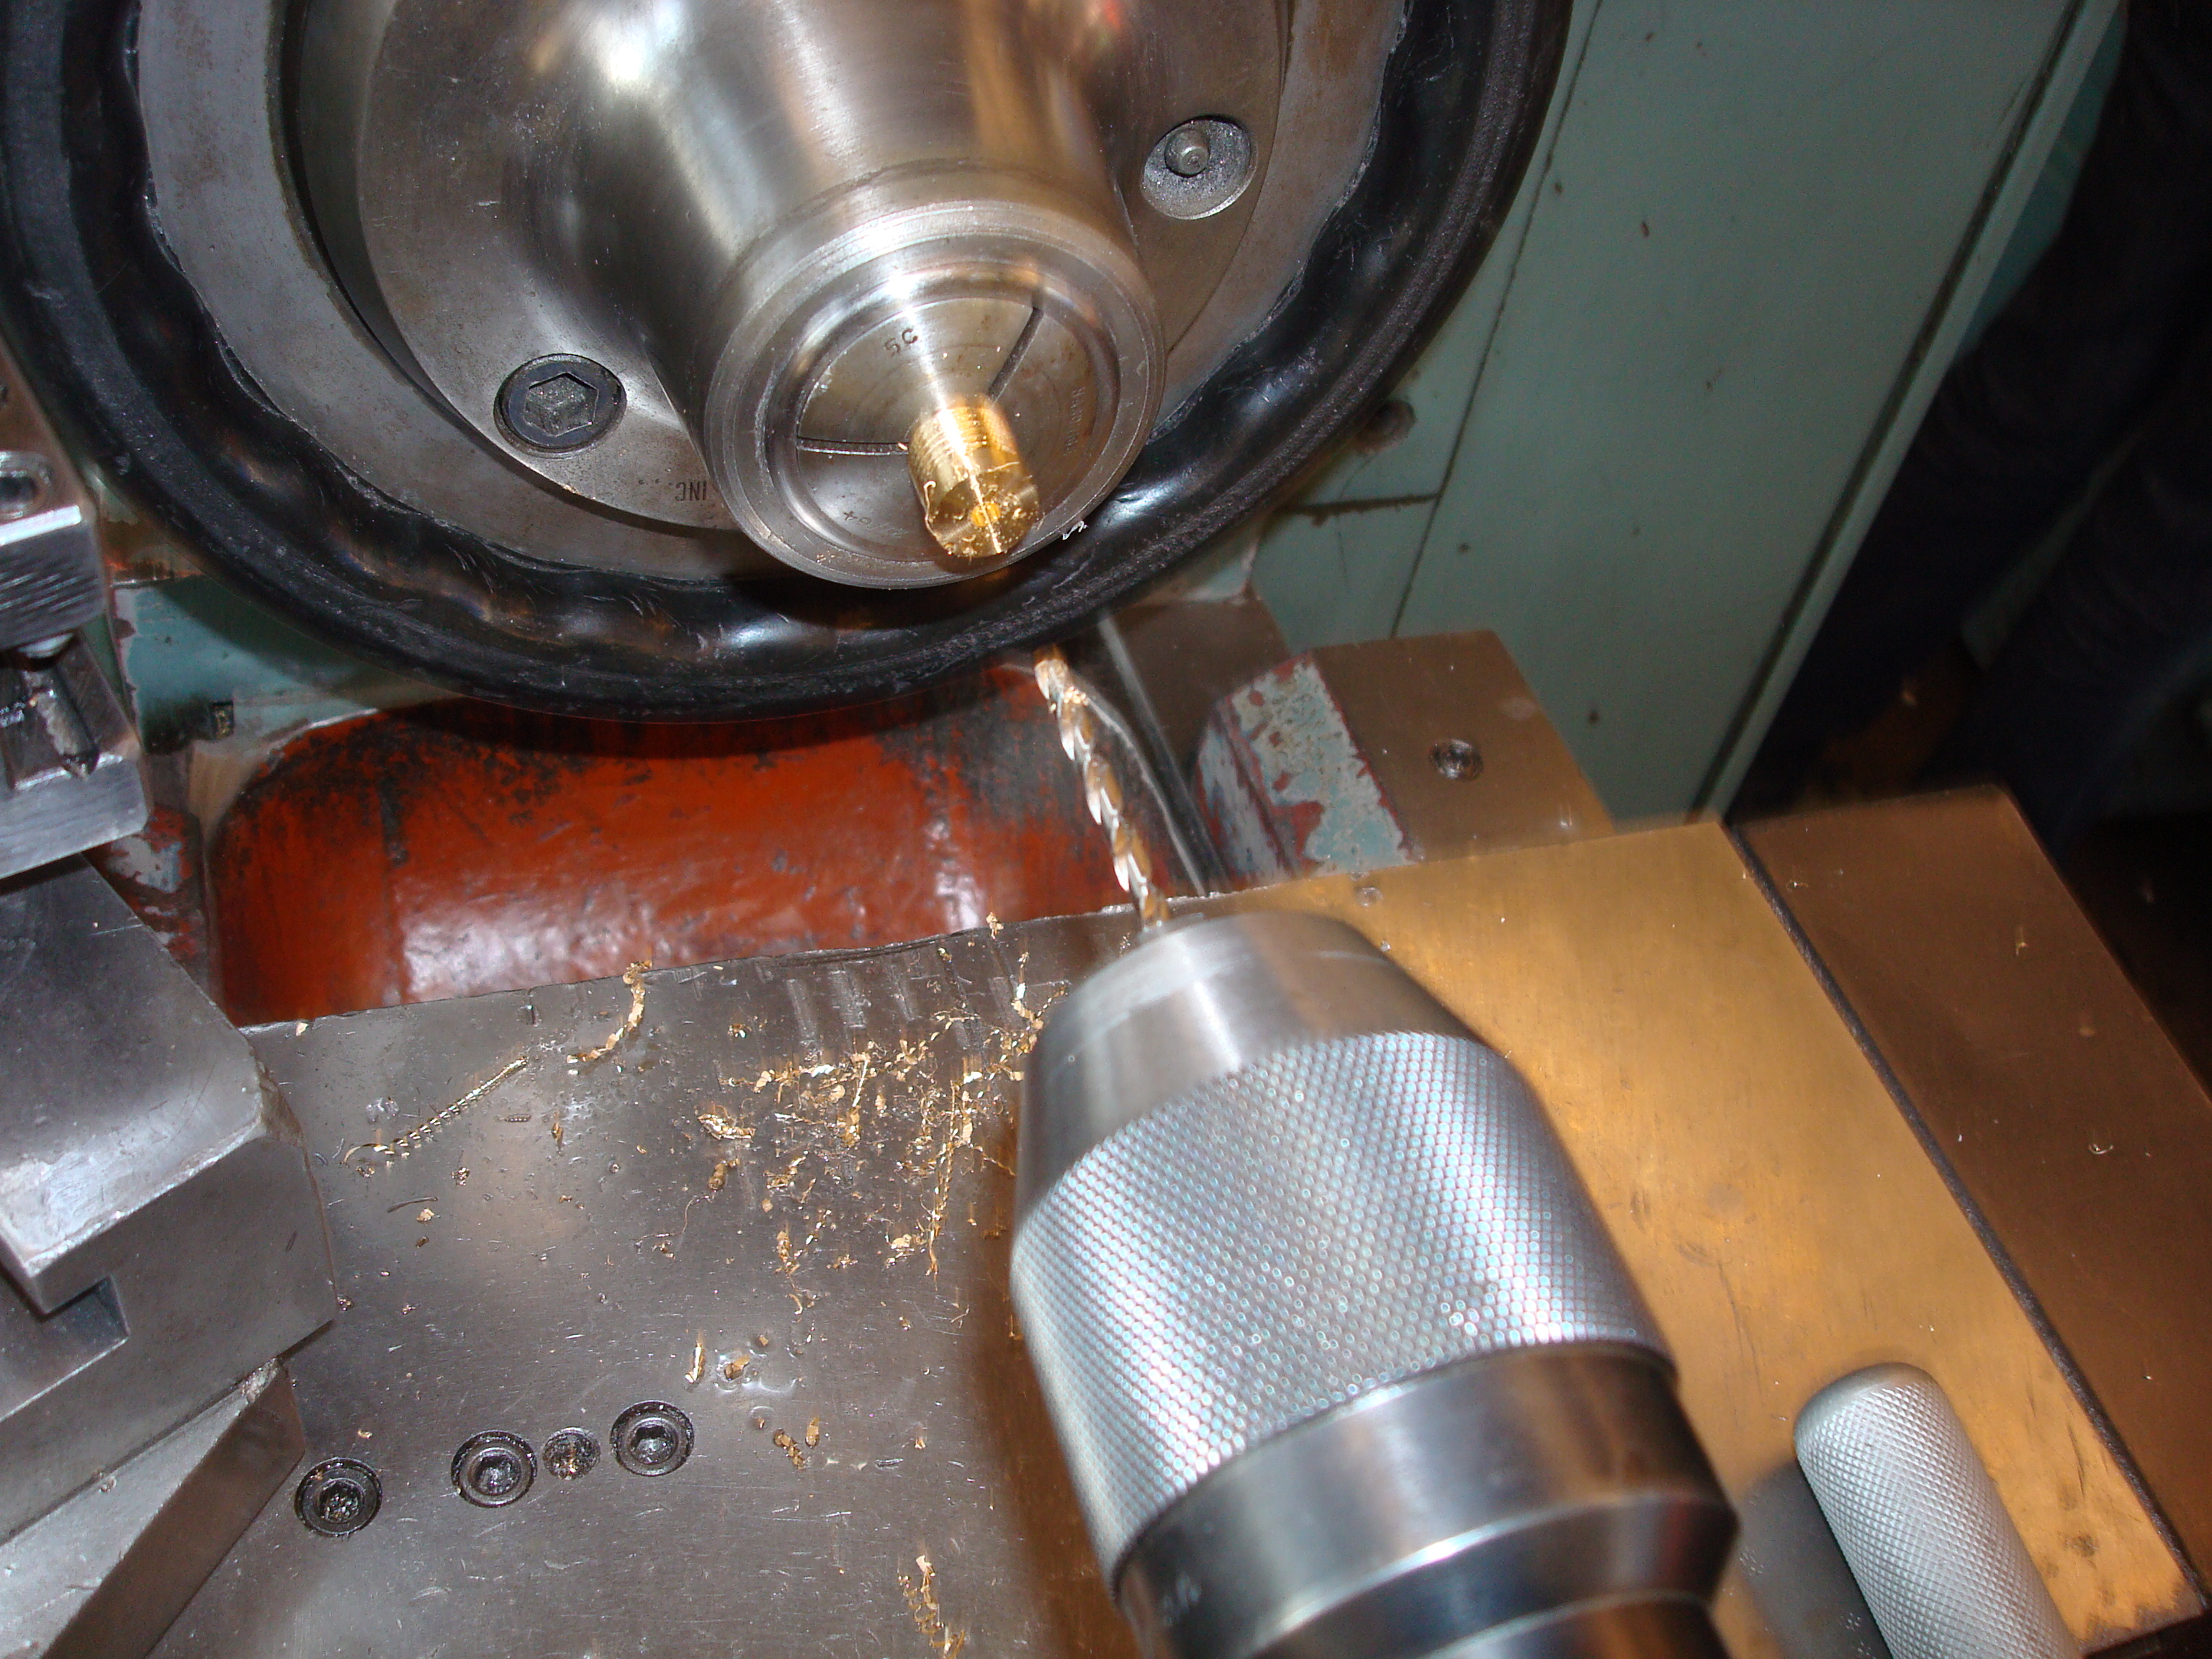
\includegraphics{concentricrodcollet.jpg}}
\end{center}
\end{itemize}
\end{itemize}

\alert{Engraving}

\begin{itemize}
\item The engravings on the dial and back sight were done by Tom and Cathy
Nyren of Tanner's Engraving in San Jose
\item The nose cone of the CNC engraver rides on the surface of the workpiece
\item The engraving tool extends .005'' below the cone and into the workpiece

\begin{center}
\scalebox{.25}{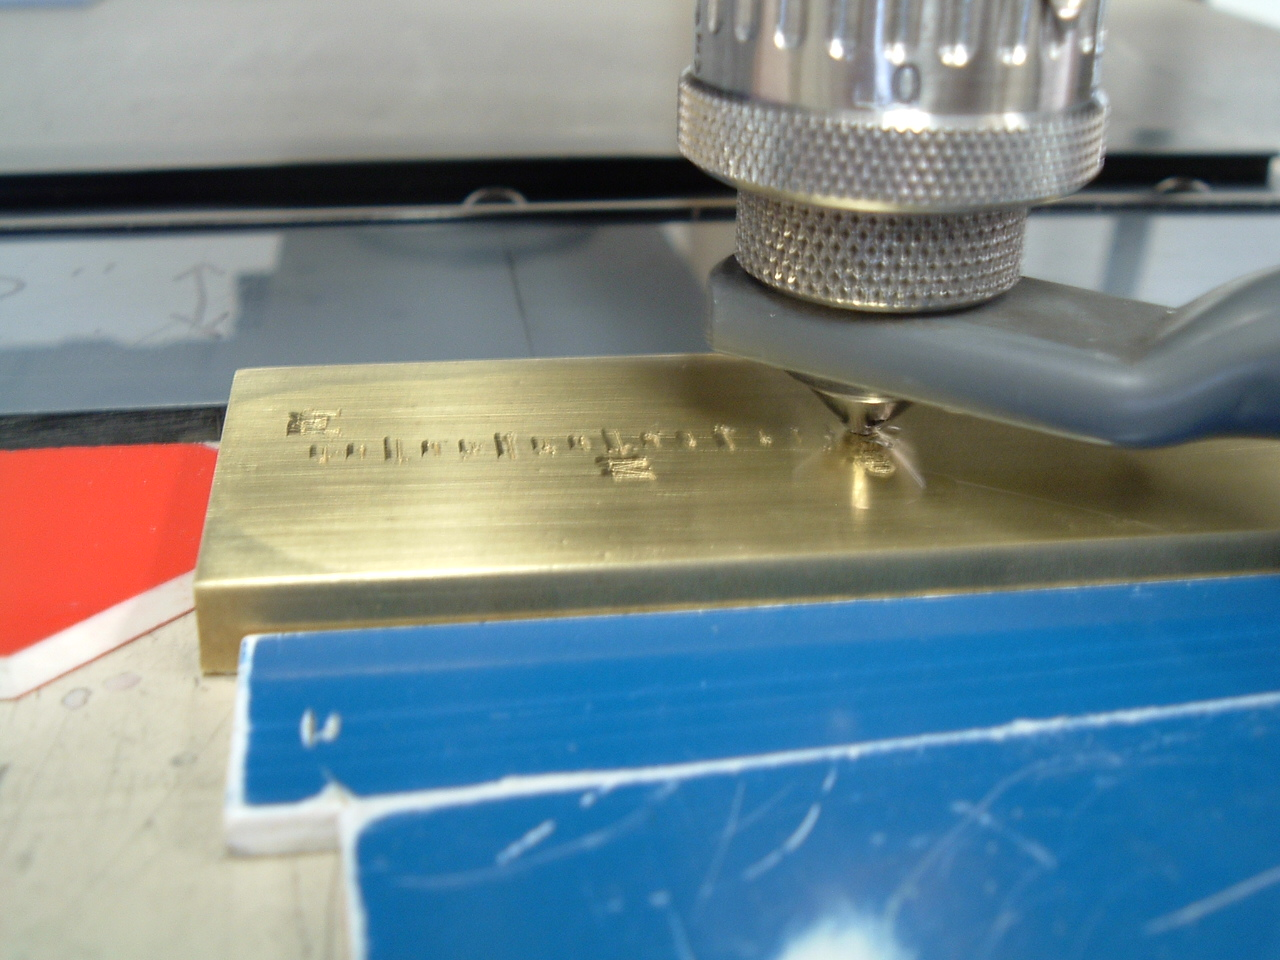
\includegraphics{engravinganalemma.jpg}}
\scalebox{.25}{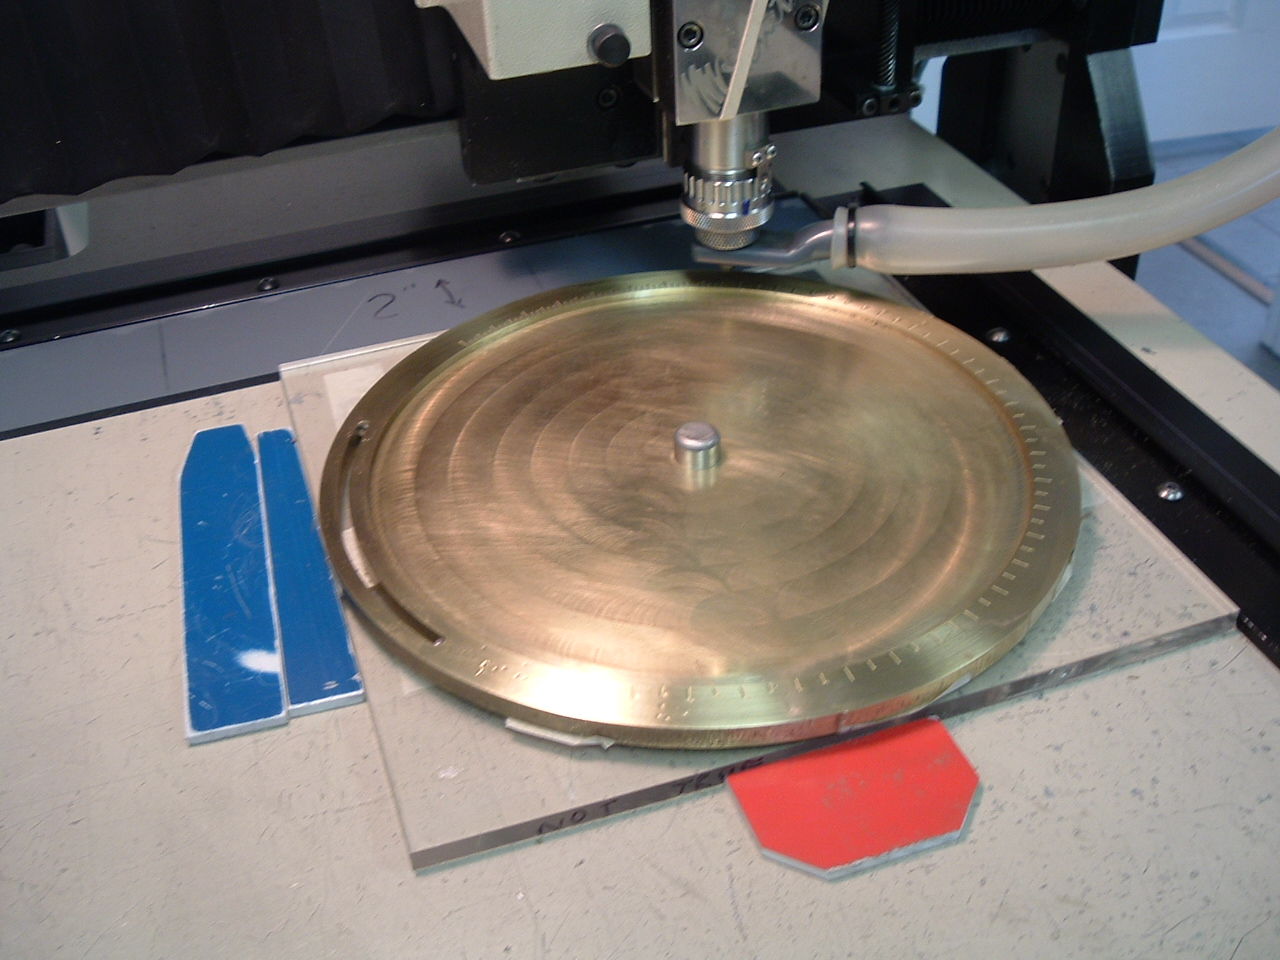
\includegraphics{engravingdial.jpg}}
\end{center}
\end{itemize}

\end{column}
\end{columns}
\end{frame}
\end{document}





